% Intended LaTeX compiler: pdflatex
\documentclass[10pt,a4paper,UTF8]{article}
\usepackage{zclorg}
\author{张朝龙}
\date{}
\title{线性映射的矩阵表示}
\hypersetup{
 pdfauthor={张朝龙},
 pdftitle={线性映射的矩阵表示},
 pdfkeywords={},
 pdfsubject={},
 pdfcreator={Emacs 25.0.50.1 (Org mode 9.0.5)}, 
 pdflang={English}}
\begin{document}

\maketitle
\tableofcontents
\titlepic{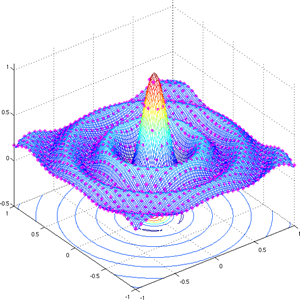
\includegraphics[scale=0.25]{../../img/sinc.PNG}}
\newpage

从同济大学的线性代数课本里第一次接触矩阵。接触矩阵之前刚刚被各种奇葩的行列式计算折磨。矩阵的到来又是一堆公式,实在让人摸不着头脑。《linear algebra done right》从线性映射出发,赋予矩阵更深层次的意义。我觉得矩阵的概念就应该从线性映射导出。

\section{矩阵与线性映射的关系}
\label{sec:org3384256}


接下来我们就用矩阵来表示线性映射。我们知道如果\(v_{1},\ldots ,v_{n}\)是\(V\)的基,且\(T:V\rightarrow W\)是线性的,那么\(Tv_{1},\ldots ,Tv_{n}\)的值确定了\(T\)在\(V\)的任意向量上的值,因为我们之前证明过 \[\dim V = \dim nullT + \dim range T\]。
马上就可以看到,利用矩阵和\(W\)的基,矩阵可以有效地记录这些\(Tv_{j}\)

\begin{definition}
设\(m,n\)是正整数,\(m\times n\)矩阵\(A\)是由\(\mathbf{F}\)的元素构成的\(m\)行\(n\)列的矩阵:
\begin{equation}
\label{eq:2}
A=
\begin{bmatrix}
A_{1,1} & \ldots & A_{1,n} \\
\vdots  & \ddots & \vdots \\
A_{m,1} & \ldots & A_{m,n}
\end{bmatrix}
\end{equation}
\end{definition}
\begin{definition}
设\(T\in \mathcal{L}(V,W)\),并设 \(v_{1},\ldots ,v_{n}\)是\(V\)的基,\(w_{1},\ldots ,w_{n}\)是\(W\)的基。规定\(T\)关于这些基的矩阵为\(m\times n\)矩阵\(\mathcal{M}(T)\),其中\(A_{j,k}\)满足:
\[Tv_{k} = A_{1,k}w_{1} + \ldots + A_{m,k}w_{m}\]
\end{definition}
线性映射\(T\in \mathcal{L}(V,W)\)的矩阵\(\mathcal{M}(T)\)依赖于\(V\)的基\(v_{1},\ldots ,v_{n}\)和\(W\)的基\(w_{1},\ldots ,w_{n}\)以及\(T\)。把\(Tv_{k}\)写成\(w_{1},\ldots ,w_{n}\)的线性组合:\(Tv_{k} = A_{1,k}w_{1} + \ldots + A_{m,k}w_{m}\) 其中的系数就构成了\(\mathcal{M}(T)\)的第\(k\)列。如果\(T\)是从\(n\)维空间到\(m\)维空间的一个线性映射,则\(\mathcal{M}(T)\)是一个\(m\times n\)矩阵。

\begin{instance}
设\(T\in \mathcal{L}( \mathbf{F}^{2}, \mathbf{F}^{3})\)定义如下:
\[T(x,y) = (x+3y,2x+5y,7x+9y)\]
则\(T\)关于\(\mathbf{F}^{2}\)和 \(\mathbf{F}^{3}\)的标准基的矩阵为:
\begin{equation}
\label{eq:1}
\mathcal{M}(T) = 
\begin{bmatrix}
1 & 3 \\
2 & 5 \\
7 & 9
\end{bmatrix}
\end{equation}
在这个例子中,我们需要从\(\mathbf{F}^{2}\) 的标准基\((1,0),(0,1)\)和\(\mathbf{F}^{3}\)的标准基构建\(T(x,y) = (x+3y,2x+5y,7x+9y)\)的映射。显然有\(T(1,0) = (1,2,7),T(0,1) = (3,5,9)\) 
\end{instance}

\begin{instance}
设\(D\in \mathcal{L}( \mathcal{P}_{3}( \mathbf{R}), \mathcal{P}_{2}( \mathbf{R}))\)是微分映射 \(Dp = p^{'}\), 求\(D\)关于 \(\mathcal{P}_{3}( \mathbf{R})\) 和 \(\mathcal{P}_{2}( \mathbf{R})\)的标准基矩阵。(在考虑\(\mathcal{P}_{m}( \mathbf{F})\)时,除非特别声明,总是用标准基\(1,x,x^{2},\ldots ,x^{m}\))
显然我们有 \(D(1) = 0, D(x) = 1, D(x^{2}) = 2x,D(x^{3}) = 3x^{2}\) ,则有:
\begin{equation}
\label{eq:3}
\mathcal{M}(D) = 
\begin{bmatrix}
0 & 1 & 0 & 0 \\
0 & 0 & 2 & 0 \\
0 & 0 & 0 & 3
\end{bmatrix}
\end{equation}
\end{instance}




\section{矩阵加法和标量乘法与线性映射的关系}
\label{sec:org6ead70b}


我们假定\(V\)和\(W\)总是有限维的,且已经确定\(V\)和\(W\)的基,对于每个从\(V\)到\(W\)的线性映射,我们都可以谈论它的矩阵(当然这个矩阵也是关于这些确定的基的。)。

首先我们探讨两个线性映射之和的矩阵是否是这两个线性映射矩阵之和。这个问题到现在还没有意义,因为我们还没有定义矩阵之和(当然这是严谨的做法,事实上,矩阵之和的定义相当简单)。
\begin{definition}
规定两个同样大小的矩阵的和是把矩阵中对应的元素相加得到的矩阵:
\begin{equation}
\label{eq:4}
\begin{bmatrix}
A_{1,1} & \ldots & A_{1,n} \\
\vdots  & \ddots & \vdots \\
A_{m,1} & \ldots & A_{m,n}
\end{bmatrix}
+ 
\begin{bmatrix}
C_{1,1} & \ldots & C_{1,n} \\
\vdots  & \ddots & \vdots \\
C_{m,1} & \ldots & C_{m,n}
\end{bmatrix}
= 
\begin{bmatrix}
A_{1,1} + C_{1,1} & \ldots & A_{1,n} + C_{1,n} \\
\vdots  & \ddots & \vdots \\
A_{m,1} + C_{m,1} & \ldots & A_{m,n} + C_{m,n}
\end{bmatrix}
\end{equation}
\end{definition}
对于\(S,T\in \mathcal{L}(V,W)\),假设\(S+T,S,T\)都采用相同的基,则有\(\mathcal{M}(S+T) = \mathcal{M}(S) + \mathcal{M}(T)\) 

\begin{definition}
规定标量与矩阵的乘积就是用该标量乘以矩阵中的每个元素
\begin{equation}
\label{eq:5}
\lambda
\begin{bmatrix}
A_{1,1} & \ldots & A_{1,n} \\
\vdots  & \ddots & \vdots \\
A_{m,1} & \ldots & A_{m,n}
\end{bmatrix}
= 
\begin{bmatrix}
\lambda A_{1,1}  & \ldots & \lambda A_{1,n}  \\
\vdots  & \ddots & \vdots \\
\lambda A_{m,1} & \ldots & \lambda A_{m,n}
\end{bmatrix}
\end{equation}
\end{definition}
假设线性映射\(\lambda T\)和\(T\)使用相同的基,则对于\(T\in \mathcal{L}(V,W)\)有 \(\mathcal{M}(\lambda T) = \lambda \mathcal{M}(T)\)

对于正整数\(m\)和\(n\),元素取自\(\mathbf{F}\)的所有\(m\times n\)的矩阵构成的集合记为\(\mathbf{F}^{m,n}\)则\(\mathbf{F}^{m,n}\)是\(mn\)维向量空间。

对于\(\mathbf{F}^{mn}\)是向量空间的证明只用参照向量空间的定义即可,另外我们可以发现对于\(\mathbf{F}^{m,n}\),某个位置为\(1\)其余位置为\(0\)的元素构成了\(\mathbf{F}^{m,n}\)的基,共有\(mn\)个这样的矩阵,所以\(\mathbf{F}^{mn}\)的维数等于\(mn\). 我们可以先证明某个位置为1,其余位置为零的矩阵张成了\(\mathbf{F}^{mn}\),然后证明这些元素是线性无关的。

\section{矩阵乘法与线性映射的关系}
\label{sec:org6e0b980}


我们假设\(v_{1},\ldots ,v_{n}\)是\(V\)的基,\(w_{1},\ldots ,w_{m}\)是\(W\)的基,并设\(U\)是另一个向量空间,\(u_{1},\ldots ,u_{p}\)是\(U\)的基。考虑线性映射\(S:U\rightarrow V, T:V\rightarrow W\),他们的复合映射\(ST\)是从\(U\)到\(W\)的线性映射。那么\(\mathcal{M}(ST)\)是否等于\(\mathcal{M}(S)\)乘以\(\mathcal{M}(T)\)呢?

对于这个问题,我们的处理方法是,找到矩阵乘法的一种合适的定义,使其满足\(\mathcal{M}(ST) = \mathcal{M}(S) \mathcal{M}(T)\)。

设\(\mathcal{M}(S) = A, \mathcal{M}(T) = C\), 则有:
\begin{eqnarray}
\label{eq:6}
(ST)u_{k} &=& S(Tu_{k})  \\
&=& S(\sum_{i=1}^{n}C_{i,k}v_{i}) \\
&=&\sum_{i=1}^{n}C_{i,k}S(v_{i}) \\
&=&\sum_{i=1}^{n}C_{i,k}\sum_{j=1}^{m}A_{j,i}w_{j}\\
&=&\sum_{i=1}^{n}\sum_{j=1}^{m}C_{i,k}A_{j,i}w_{j} \\
&=&\sum_{j=1}^{m}\sum_{i=1}^{n}(A_{j,i}C_{i,k}) w_{j}
\end{eqnarray}
因此\(\mathcal{M}(ST)\)是\(m\times p\)矩阵,它的第\(j\)行第\(k\)列元素等于\(\sum_{i=1}^{n}A_{j,i}C_{i,k}\)
\begin{definition}


设\(A\)是\(m\times n\)矩阵,\(C\)是\(n\times p\)矩阵,\(AC\)定义为\(m\times p\)矩阵,其第\(j\)行第\(k\)列元素是\[(AC)_{j,k} = \sum_{i=1}^{n}A_{j,i}C_{i,k}\]

即,把\(A\)的第\(j\)行和\(C\)的第\(k\)列的对应元素相乘再求和就得到\(AC\)的第\(j\)行第\(k\)列元素。从定义我们也可以看出只有当一个矩阵的列数等于第二个矩阵的行数的时候才可以进行矩阵乘法计算。另外我们还可以发现,对于\(1 \leq k \leq p\)有\((AC)_{\cdot,k} = AC_{\cdot,k}\),即\(AC\)的第\(k\)列等于\(A\)乘以\(C\)的第\(k\)列。我们可以把这个过程当做\(C\)中第\(K\)列的元素和\(A\)中各个列构成的线性组合。
\end{definition}
假设考虑\(T\in \mathcal{L}(U,V)\)和\(S\in \mathcal{L}(V,W)\)时使用\(V\)的同一基,在考虑\(S\in \mathcal{L}(V,W)\)和\(ST\in \mathcal{L}(U,W)\)是使用\(W\)的同一基,在考虑\(T\in \mathcal{L}(U,V)\)和\(ST\in \mathcal{L}(U,W)\)是使用\(U\)的同一基,有\(\mathcal{M}(ST) = \mathcal{M}(S) \mathcal{M}(T)\)
\end{document}
